\documentclass[bigger]{beamer}

\usepackage{booktabs}
\useinnertheme{rounded}
\usecolortheme{crane}
\setbeamerfont{block title}{size={}}
\usepackage[autolanguage]{numprint}

\usetheme{Proso}

\title{Impact of Question Difficulty on Engagement and Learning}

\author{Jan Papou\v{s}ek, \textbf{V\'it Stanislav}, Radek Pel\'anek \\
%Masaryk University Brno\\
%Czech Republic
}

\date{ITS 2016}
 
\begin{document}

\frame{\titlepage}

\begin{frame}
  \frametitle{Example scenario}
	\noindent\makebox[\textwidth]{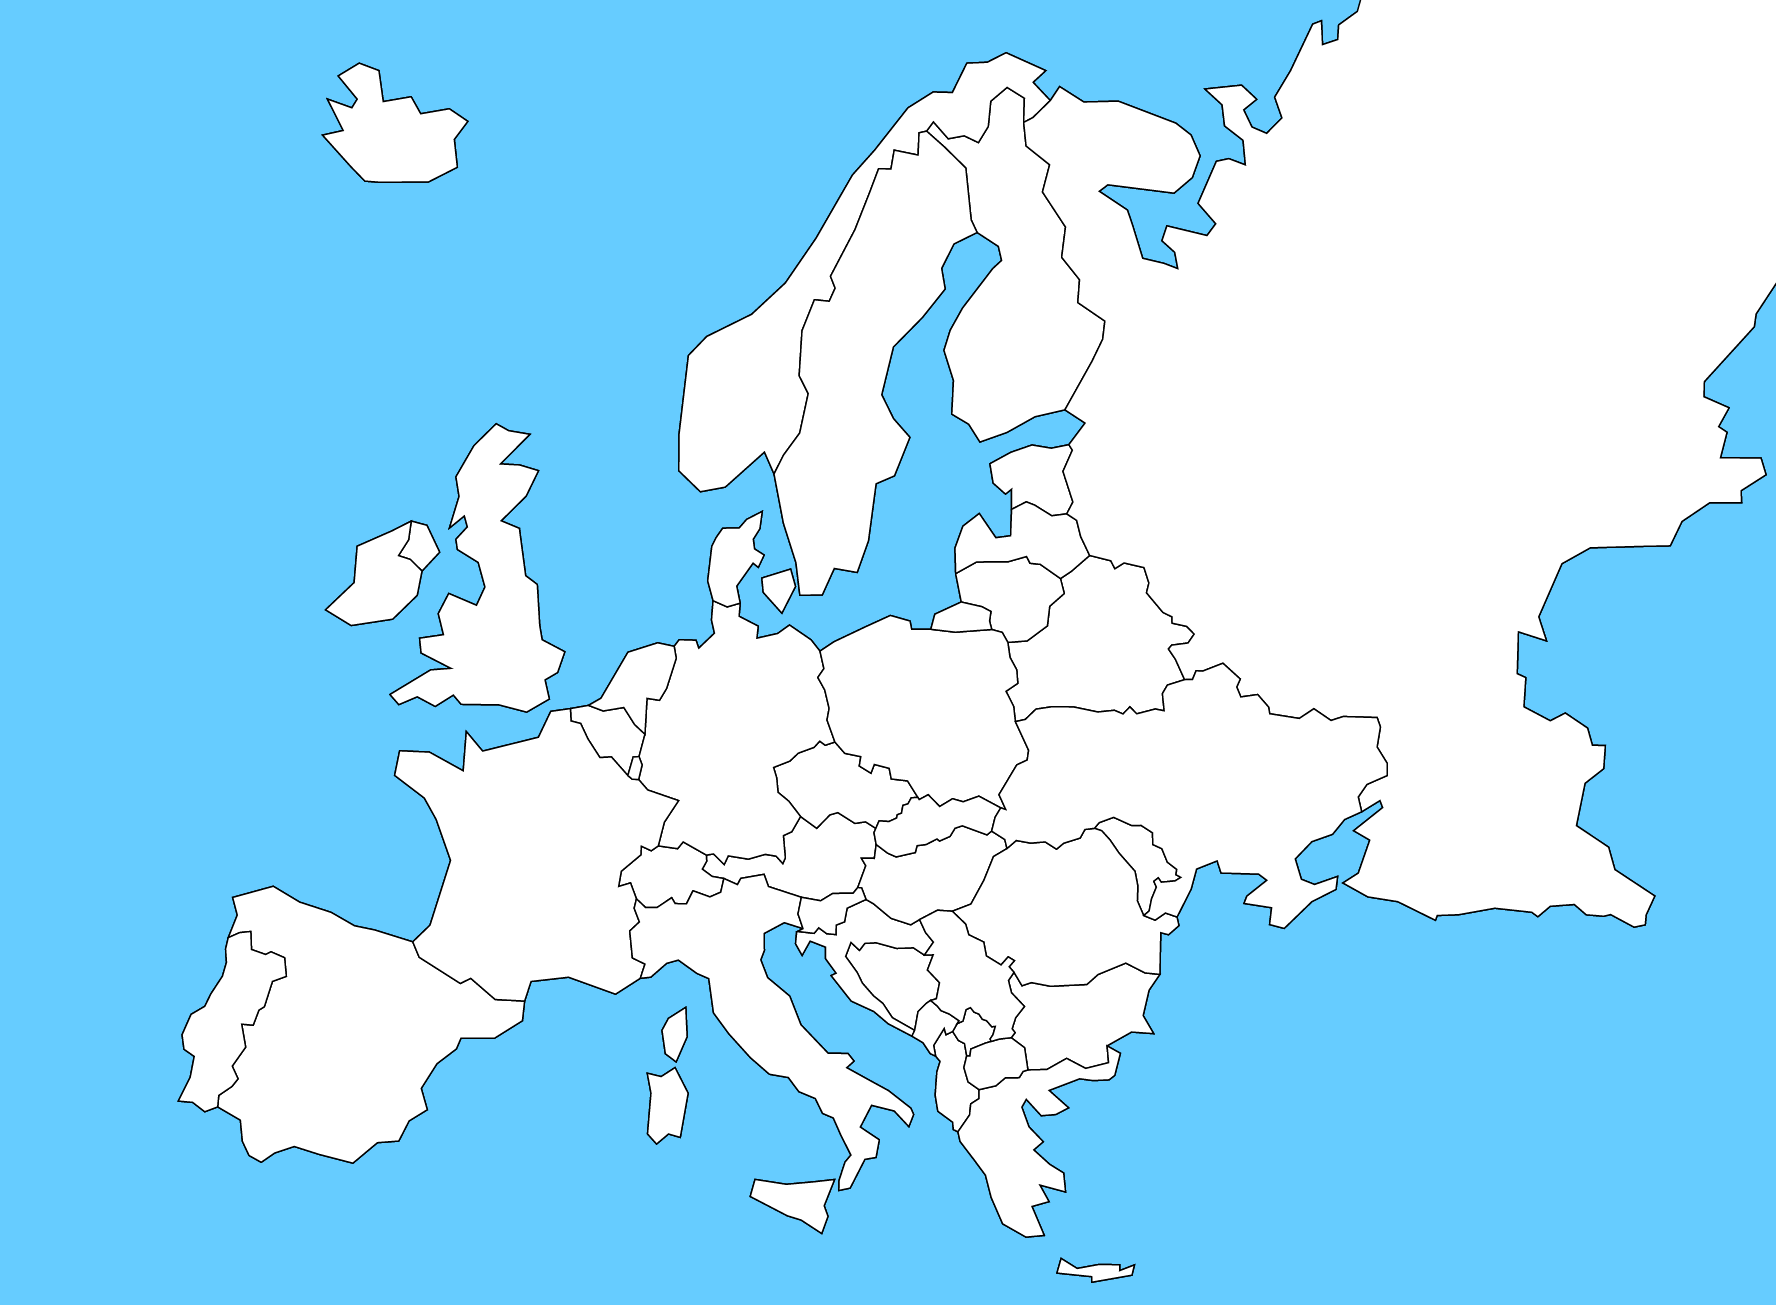
\includegraphics[width=\paperwidth]{img/europe-state}}
\end{frame}

\begin{frame}
  \frametitle{Example scenario}
	\begin{itemize}
	  \item Want to learn some facts
		\item Two scenarios (TODO vizual): \\
		A) 90\% success rate \\
		B) 50\% success rate
	\end{itemize}
\end{frame}

\begin{frame}
  \frametitle{Research question}
	\begin{center}
    {\Huge What is optimal question difficulty?} 

		\medskip
    ...for engagement and learning
	\end{center}
\end{frame}

\begin{frame}
  \frametitle{Our setting}
	\begin{itemize}
		\item 
	\end{itemize}
\end{frame}

\begin{frame}
  \frametitle{}
	\begin{itemize}
		\item 
	\end{itemize}
\end{frame}

\begin{frame}
	\frametitle{outlinemaps.org}
	\only<1>{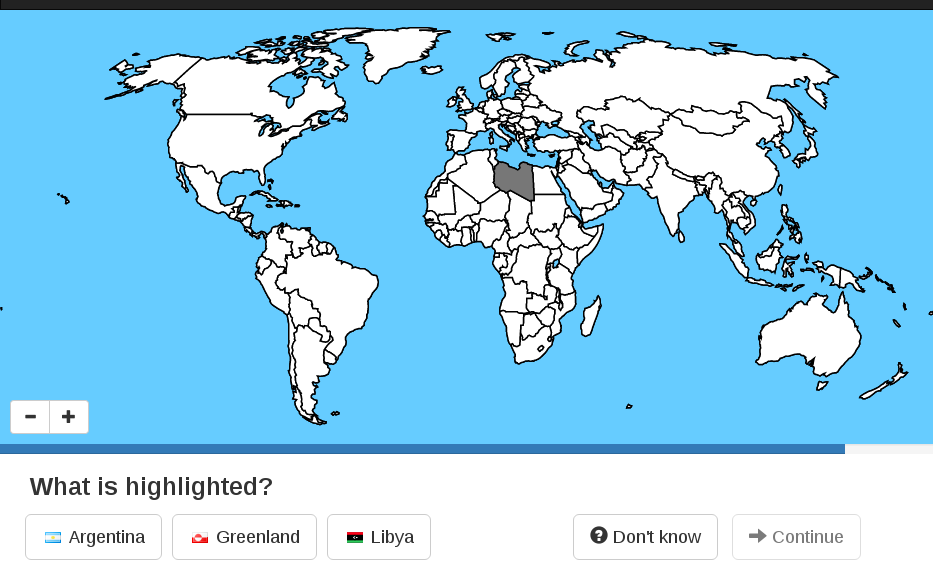
\includegraphics[width=\textwidth]{img/slepemapy_world_practice}}
	\only<2>{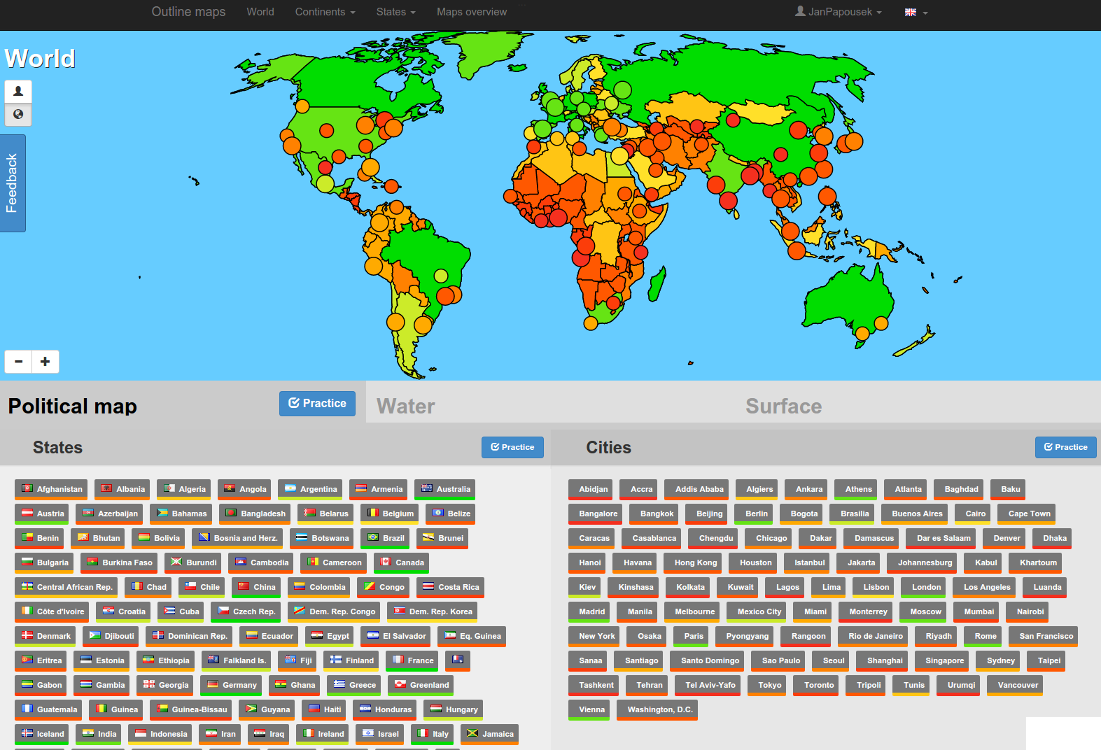
\includegraphics[width=\textwidth]{img/slepemapy_world}}
\end{frame}

\begin{frame}
  \frametitle{Experimental setting}
	\begin{itemize}
		\item online AB experiment
		\item new users were randomly assigned to one of the studied conditions
	\end{itemize}
	\begin{center}
		\begin{tabular}{ccc}
			\textbf{Target error rate} & \textbf{notation} \\
			\toprule
			 5\% & C05 \\
			 20\%   & C20 \\
			 35\% & C35 \\
			 50\%   & C50 \\
			\bottomrule
		\end{tabular}
	\end{center}

\end{frame}

\begin{frame}
	\frametitle{Experimental Setting}
	\begin{itemize}
		\item November 2015 to January 2016
		\item \numprint{3300000} answers from \numprint{37000} learners
		\item majority of users:
			\begin{itemize}
				\item Czech Republic (84 \%)
				\item Slovakia (8 \%)
			\end{itemize}
	\end{itemize}
\end{frame}

\begin{frame}
  \frametitle{Engagement}
	\begin{itemize}
		\item 
	\end{itemize}

\end{frame}


\begin{frame}
  \frametitle{Learning}
	\begin{itemize}
		\item 
	\end{itemize}

\end{frame}


\begin{frame}
  \frametitle{Conclusion}
	\begin{itemize}
		\item 
	\end{itemize}

\end{frame}




\begin{frame}
	\begin{center}
		{\Huge outlinemaps.org}

		\medskip
		(data.outlinemaps.org)

		\bigskip
		\bigskip
		slaweet@mail.muni.cz
	\end{center}
\end{frame}
\end{document}

